%
\documentclass[11pt]{thesis} % draft

\title{Algorithmic Meta-Creativity}
\author{Fania Raczinski}
\date{March 2015}

% Test

\begin{document}

\subsubsection{Manipulation}

Within the manipluation category, (different representations of) sounds are pataphysicalised directly. There are several approaches to this, such as making changes to sound wave forms (an antinomy pataphysicalisation for example could be to invert a sound wave, i.e. where there was silence there is now noise and vice versa). These manipulations could be applied to specific sections only or the complete sound wave. This kind of manipluation could also be applied to musical scores. Changes might also happen in given compositions of music of multiple instruments (as opposed to pataphysicalising the composition process itself which is covered in section~\ref{s:composition}\marginpar{§~\ref{s:composition}}).

\begin{figure}[!htbp]
\centering
  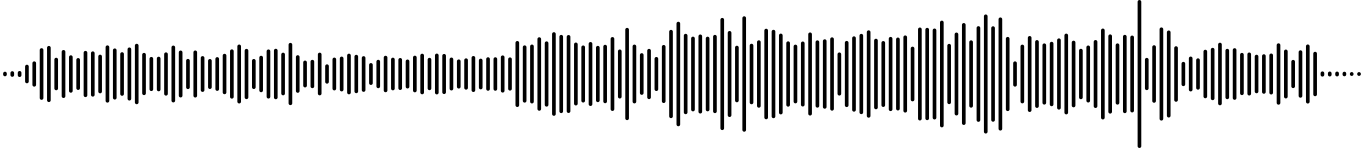
\includegraphics[width=\linewidth]{simplewave.pdf}
\caption[Sound wave of \textit{La Chanson Du D{\'e}cervelage}]{Sound wave of \textit{La Chanson Du D{\'e}cervelage} \autocite[][Track 1]{UbuWebPata} (generated using \autocite{Heesakkersnd})}
\end{figure}

Various tools might be useful for these sorts of manipulations, including the \textit{Web Audio API} by the \ac{W3C} \autocite{Adenot2017}. It includes ``capabilities found in modern game audio engines as well as some of the mixing, processing, and filtering tasks that are found in modern desktop audio production applications'' \autocite*{Adenot2017}. An example of using this API to synthesise sounds is described in \autocite{Misuary2016}. Other \ac{API}s such as SoundCloud \autocite{soundcloud} might be helpful as well. 

Another approach altogether could be to play with \ac{MIDI} \autocite{midind} but this needs to be explored a lot further.


\subsubsection{Search}

Similar to the image and video search of \url{pata.physics.wtf}, audio search could be based on tags provided through an \ac{API} such as FreeSound \autocite{freesoundnd}. 

\begin{quotation}
  The query does a weighted search over some sound properties including sound tags, the sound name, its description, pack name and the sound id. Therefore, searching for query=123 will find you sounds with id 1234, sounds that have 1234 in the description, in the tags, etc. \sourceatright{\autocite{freesoundnd}}
\end{quotation}

The search would work in a similar way then. Section~\ref{s:imgvid}\marginpar{§~\ref{s:imgvid}} specifies that we (1) translate query, (2) pataphysicalise the translation, and (3) retrieve matching images/videos using \ac{API} calls.

So, say the user query is `rumbling', that would be translated to `grondant' (French for `growling') and `\begin{CJK}{UTF8}{min}お叱り\end{CJK}' (Japanese for `scold') and finally the English `scolding'. From this we then produce a list of 10 patadata (`[berate, chide, call on the carpet, chiding, rag, lambast, bawl out, tongue-lashing, grouch, scold]') by pataphysicalising this translated term. This patadata is then used to actually retrieve sound files through an \ac{API}.

Issues that can arise with the use of external \ac{API}s and folksonomy (user generated tags) have already been mentioned in section~\ref{s:apis} and~\ref{s:imgalgoimprovs}\marginpar{§~\ref{s:apis}}. With sound files specifically perhaps tags might be very subjective. This may or may not be useful in a pataphysical context of course.


\subsubsection{Composition}
\label{s:composition}

Rather than pataphysicalising existing pieces of sound or music, this process could be applied during composition as well. This might come in the form of pataphysical constraints, inspired by \ac{OULIPO} techniques (see~\ref{s:patalipo}\marginpar{§~\ref{s:patalipo}}). In fact, there is the `OUMUPO', which deals with ``potential compositional systems or methods, potential performance, and historical research'' \autocite{Mathews2005}.

\begin{quotation}
  The creation of new forms in music is not guaranteed by the devising of new systems or procedures, since musical form is such a complex and sustracted thing in itself. The system of tonality, for example, operates by means of a set of dynamic interrelationships between tonal centres and motivic ideas which musical analysis constantly struggles to articulate. The very impossibility of defining this system once and for all is what guarantees its survival. Music strives to be free from contsrtaint. \sourceatright{\autocite{Mathews2005}}
\end{quotation}

The idea of applying chance (clinamen) was already explored by Mozart in 1787 with his \textit{Musikalisches W\"{u}rfelspiel} (``Musical Dice Game'') \autocite{Aldenhovelnd}, which allows for a total of $11^{16}$ different compositions. This is even more than Queneau's $10^{14}$ poems discussed in chapter~\ref{s:queneau}\marginpar{§~\ref{s:queneau}}.


\section{From the Aspirations to Paris by Sea}

\begin{figure}[!htb]
\centering
  \includegraphics{aspi.pdf}
\end{figure}

This chapter not only suggests work-arounds or solutions to some of the issues and problems introduced in chapter~\ref{ch:analysis} \anal~ but also proposes new additions to the system. This also includes thoughts on a potential integration of Dennis' `search and replace' algorithms from the \nameref{s:dennis} \appli~ chapter. A lot of the suggestions here refer back to topics in the \nameref{ch:implementation} \imple~ chapter, such as the index data structure, the patalgorithms for text, image and video search and the visual design elements of \url{pata.physics.wtf}. Audio is addressed in section~\ref{s:audio} \aspi~, highlighting the connection of pataphysics (see also §~\ref{ch:pataphysics}) and music first and then exploring potential pataphysicalisations of sound and music.

\begin{figure}[!htb]
\centering
  \includegraphics[width=\textwidth]{legend.pdf}
\end{figure}

\end{document}
